%\documentclass[prb,preprint,showpacs,superbib]{revtex4}

\documentclass[prl,twocolumn,showpacs,twocolumngrid,superbib]{revtex4}


\usepackage{graphicx}
\usepackage{amsfonts}
\usepackage{amsmath}
\usepackage{bm}
\usepackage{alltt}
\usepackage{fancyhdr}
\newcommand{\bms}[1]{{\boldsymbol #1}}
\renewcommand{\thefootnote}{\fnsymbol{footnote}}

%\draft
%\tighten
\pagestyle{fancy}

\begin{document}

\title{
Linear Scaling Geometry Optimization of Large Molecules by Fitting
Internal Coordinate Gradients \footnotemark[1]}

\author{K\'aroly N\'emeth\footnotemark[2]}
\author{Matt Challacombe}

\affiliation{Theoretical Division, Los Alamos National Laboratory, Los Alamos, NM 87545, USA}

\date{\today}

\begin{abstract}
{
This article peresents a new and efficient alternative to well established
algorithms for molecular geometry optimization.   The new approach 
exploits the approximate decoupling of vibrational modes in a curvilinear 
internal coordinate system,  allowing seperation  of the 3$N$-dimensional
optimization problem into an ${\cal{O}}(N)$ set of quasi non-interacting
one-dimensional problems.  Each  uncoupled optimization is developed by fitting 
energy gradients in the internal coordinate system followed by root finding.  
This new approach is competitive with the best  geometry optimization algorithms 
in the literature, achieves superlinear convergence and works well for large 
biological problems with complicated hydrogen bonding network 
and ligand binding motifs.  
}

\smallskip
\noindent{\bf Keywords}: 
geometry optimization, linear scaling, 
curvilinear internal coordinates, fitting
\end{abstract}
 

\maketitle

\footnotetext[1]{LA-UR-04-1097}
\footnotetext[2]{\tt KNemeth@LANL.Gov}

\section{Introduction}

Recently, $N$-scaling electronic structure algorithms ($N$ is the system size)  have 
realized their promise, delivering energies and forces on nuclei for large systems at 
both a numerical accuracy and theoretical level suitable to begin addressing many complex 
problems.  For example, it is now possible to routinely apply hybrid Hartree-Fock/Density 
Functional theory to fragment models in molecular biophysics involving complicated 
hydrogen bonding network and metal-ligand binding motifs 
with several hundred atoms using basis sets of triple-zeta plus 
polarization quality.  However, despite favorable scaling properties, ${\cal O}(N)$ 
methods typically carry a larger cost prefactor than their conventional counterparts.  Thus, 
in addition to parallelism, developing efficient algorithms to drive the core engines of 
linear scaling electronic structure theory is paramount.  Of these, perhaps the most useful 
driver of electronic structure theory is the molecular geometry optimizer, which follows 
the energy gradient downhill to a local minimum.   

This paper presents a new concept for the optimization of molecular 
geometries based on the approximate separability of 
curvilinear internal coordinate motions
and the recent availability of internal coordinate technology 
for large molecules
\cite{paizs_coordtrf1,nemeth_coordtrf1,paizs_coordtrf2,nemeth_coordtrf2}.  
Internal coordinates represent motions along chemical entities 
such as bond stretchings, valence angle bendings 
and torsions. In terms of internal coordinates,
interaction constants of the Hessian and higher order 
energy derivative matrices are usually an order of 
magnitude smaller than the diagonal ones 
\cite{pulay_69,fogarasi_diaghess,Pulay_natural_internals,pulay_review,pulay_dynamics}.
This is the basis for the approximate decoupling of molecular motions
in terms of internal coordinates.

An observation central to 
the present contribution is that internal coordinate gradients 
show recognizable trends during geometry optimization, 
and these trends can be formalized by curve-fitting.
The roots of the fitted curves provide a new, improved
aproximation for the location of the extrema during geometry optimization.
Such a trend is illustrated in Fig.~\ref{NH3outp6}, 
showing a typical progression of 
internal coordinate gradients and how a fitted line can predict the location
of the minimum.

\begin{figure}[h]
\resizebox*{3.5in}{!}{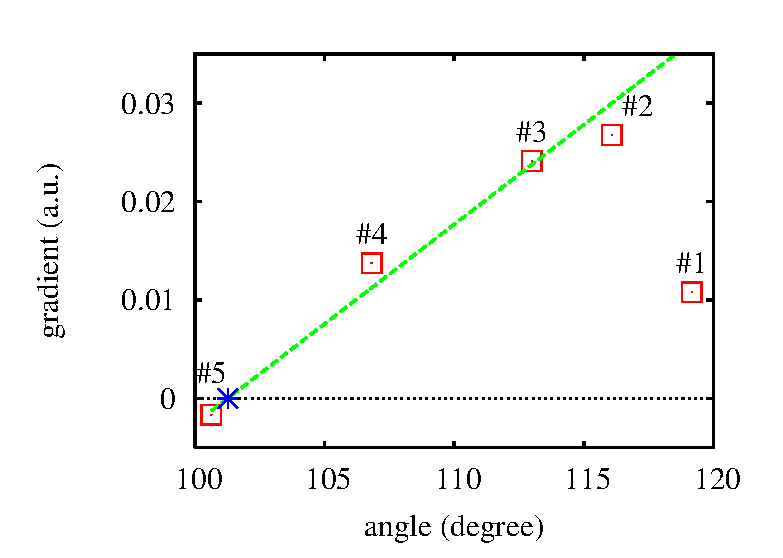
\includegraphics{picture1_2.eps}}
\caption{
Progression of gradients on a valence angle bending coordinate of
ammonia. Energies and forces were obtained by the PBE 
density functional model in STO-3G basis set.
The optimization was started from near planar geometry, i.e.
from the vicinity of a transition state, and converged to a local 
minimum of the potential energy surface. The numbers in the picture
indicate the sequence of optimization steps. The dashed line represents
a linear fit, the star the predicted location of the minimum.}
\label{NH3outp6}
\end{figure}

\pagebreak

We therefore propose solving the $3N$-dimensional molecular geometry 
optimization problem as a set of $N_{\rm int}$  
quasi-uncoupled one-dimensional 
optimization problems, where $N_{\rm int}$ is the number of internal 
coordinates. Since internal coordinates which represent chemical
concepts are well localized, $N_{\rm int}$ is proportional to $N$, the number of
atoms. This allows for constructing an optimization scheme 
which scales linearly with the system-size.
All these one-dimensional optimization problems are then treated similarly
to the one of Fig.~\ref{NH3outp6}, i.e. the location of the extrema
are determined by curve-fitting.

\subsection{Conventional Methods}
As mentioned above, internal coordinates minimize both harmonic, and
more importantly, anharmonic vibrational couplings 
\cite{pulay_69,fogarasi_diaghess,Pulay_natural_internals,pulay_review,pulay_dynamics}.
This fact provides internal coordinates with a great advantage 
in molecular
geometry optimization \cite{Pulay_natural_internals} 
and molecular dynamics \cite{pulay_dynamics}, as opposed to Cartesians.
Since Cartesian coordinates are highly coupled, a large displacement
on one coordinate may generate a large gradient on the other one
and thus delays convergence and causes oscillations. 
Not even the use of an accurate Hessian can cure this situation,
since large Cartesian displacements will induce the same effect 
as before, via anharmonic
coupling. An excellent discussion of this issue can be found in 
the Introduction of Ref.~\cite{Pulay_natural_internals}.
By this, it should be clear, that only internal coordinates 
allow large steps on the potential energy surface of molecules.
As a consequence, the use of internal coordinates can dramatically
reduce the number of optimization steps, as compared to Cartesian ones,
and is definitely the choice of coordinate systems for geometry optimization
with expensive energy and gradient evaluations, such as {\it ab initio}
calculations. This is even more valid for the optimization
of large molecules.

In the last three decades internal coordinate algorithms 
became standard, well established tools for geometry optimization 
in quantum chemistry. A recent review and comparison 
of these algorithms and their technical
details can be found in Ref.~\cite{bakken}.

All this optimization algorithms follow the Newton-Raphson scheme:
\begin{equation}
q_{i+1} = q_{i} - H^{-1} g_{i} ,
\end{equation}
where $g_{i}$ is the gradient vector, $H$ is the Hessian and
$q_{i}$ the coordinate vector of the system in the $i$-th step.
The models which use an approximate Hessian are called the
quasi-Newton techniques \cite{RFletcher}. 

A diagonal or semidiagonal approximation of the Hessian offers one
of the simplest choices to optimize geometry.
This family of techniques are often referred to as "force relaxation" 
methods.
In this case, diagonal or semidiagonal force constants are approximated
by spectroscopic values or by empirical force-fields \cite{pulay_69,pulay_review,sellers,fogarasi_diaghess,Pulay_natural_internals,van_alsenoy_98,lindh}.
Key to the success of these schemes is an appropriate choice of the
diagonal force-constants. In a complicated biomolecule, with 
an extended hydrogen bonding network and occasionally metal-ligand bonds the
variety of bonds is so large, that it is very difficult to find appropriate
force constants for each bonds. In spite of these difficulties, the biggest
{\it ab initio} geometry optimization in the literature, the geometry 
optimization of Crambin, has been carried out using the force 
relaxation technique. This optimization,
carried out by Van Alsenoy \cite{van_alsenoy_98}, used a 
relative small basis set, 4-21G and the {\it ab initio} Hartree-Fock model.
The electronic structure code has been reported to scale linearly with 
system size. The scaling of the optimizer has not been reported, it was
probably at least cubic, due to the lack of appropriate coordinate 
transformations. The crystal structure has been optimized in 79 steps
by the internal coordinate optimizer.

It is important to mention, that the steps calculated by 
force relaxation are often strongly damped, in order to avoid divergence
\cite{sellers}. One way of damping the steps, that can be used in general,
not just for force relaxation, is the line search \cite{sclegel_linesearch}.
The essence of a line search is, that once a bad step is observed by an 
increase of the energy an interpolation between Cartesian structures takes 
place, to reduce the stepsize and find a lower energy structure. 
Usually no gradient evaluation takes place during the line search, thus
the line search is not counted as an optimization step.

Another important technique to control and accelarate convergence of geometry
optimization is the geometric DIIS \cite{Pulay_GDIIS} (GDIIS). Geometric DIIS is
seems to be a simple technique, however its successful application needs
to take care of many intricate details \cite{Farkas_GDIIS}.
For this reason, simple implementations do not always succeed \cite{bakken}.
Still the technique counts as one of the standard algorithms of the field
\cite{fogarasi_diaghess,Pulay_natural_internals,eckert,Farkas_GDIIS}.
Most successful force relaxation methods either used damping, line-search,
or GDIIS, or combinations of them. 

In order to avoid the empirism related to the choice of approximate diagonal
Hessians and to have explicite account of the
coupling force constants, the use of Hessian matrix update techniques
\cite{RFletcher} emerged also in quantum chemistry. For a list
of some of the most important practical choices of update
techniques see Ref.~\cite{bakken}. 
The most frequently used updating method in molecular geometry optimization
is the Broyden-Fletcher-Goldfarb-Shanno (BFGS) technique \cite{RFletcher}
A rough guess of the Hessian, usually a
diagonal approximation, is set up in the first optimization step, in Cartesian
representation. This guess is then updated at each new optimization step
using Cartesian displacement and gradient vectors from past optimization steps.
The update matrices are of rank-1 or rank-2 type \cite{RFletcher}. 
In order to utilize internal coordinates in connection with the updated
Cartesian Hessians, the Cartesian Hessian matrices are transformed into
internal coordinate representation at each optimization step \cite{bakken}.

It is important to note, that it is technically difficult to 
update Hessians in internal coordinates, if the definition of 
the internal coordinates changes during the course of the optimization. 
Since the Cartesian Hessian matrix is usually much less sparse then the 
internal coordinate one, it is more difficult to treat it by sparse matrix 
techniques, which would allow linear scaling operation count during the
optimization steps. In the approach of Stewart \cite{Stewart_crambin_opt}
the updated inverse Hessian was stored in a sparse matrix fashion to
optimize the structure of crambin on the PM3 semiempirical level of theory. 
The approach used mixed Cartesian-internal
coordinate system, due to the lack of linear scaling coordinate transformations.
The reported efficiency of the algorithm was rather poor.

There have been some other approaches to reduce the operation
count of geometry optimization steps. Schlegel and Farkas developed
a quadratically scaling scheme to carry out coordinate transformations
and step-vector calculations in the framework of the rational function 
optimization scheme \cite{schlegel_on2iter}. Bofill {\it et.al.} 
applied Lanczos algorithm for a similar problem \cite{bofill_lanczos}.

Daniels {\it et.al.} \cite{Schlegel_plasminogen_opt} optimized the
structure of an 80 aminoic acid protein, Kringle 1, by the semiempirical 
PM3 technique, using a linear scaling PM3 code and the quadratically scaling
optimizer of Schlegel {\it et.al.} \cite{schlegel_on2iter}. 
Initial structures were taken from the crystallographyc data bank and
refined by molecular mechanics optimization. The resulting structure 
served as a starting point for the PM3 optimization, which converged in 
362 steps.

Merz {\it et.al.} used Cartesian coordinates to optimize several large 
proteins, such as AFP, crambin and Kringle1 \cite{merz_divc_geomopt} using
the PM3 semiempirical level of theory.
The structures have been refined first by molecular mechanics optimization,
then by PM3. The Cartesian optimizer was driven by
the limited memory BFGS algorithmm of Nocedal {\it et.al.} (LBFGS) 
\cite{nocedal_lbgs}. LBFGS is a simplified version of the BFGS, which scales
linearly with the system size, as opposed to BFGS. The quality of the 
approximate LBFGS Hessian is much more crude than the one of BFGS, which 
usually ends up in a larger number of optimization steps, than BFGS.

Summarizing all the above efforts, there has been considerable work
put in reducing the operation count of optimizers and extending the 
applicability of electronic structure methods to the optimization of
large molecules.

Our contribution in the present paper focuses on the applicability of
internal coordinate geometry optimization of large molecules. Particularly,
on the reduction of scaling in the optimizer. We will show, that a new
concept of geometry optimization, which does not use any of the Hessian update
techniques can provide efficiency and linear scaling for the optimization
of both small and large molecules, while using only first order energy 
derivatives.

\section{A new concept}

In the present article we introduce a new concept 
to molecular geometry optimization. We call this approach the
Extrapolation of Fitted Internal coordinate
Gradients for the localization of Extrema (EFIGE).
This new approach is very simple to implement, scales fully linearly with system size 
and is very efficient for both small and large molecules.

The new algorithm is based on the fact that
normal mode gradients are linear functions of the normal mode values 
on harmonic potential energy surfaces. 
In the process of geometry optimization the goal is to reveal the roots
of these lines, where all gradients become zero. In order to 
find these roots, first a few points should be determined from each
lines, then the roots can be revealed by line-fitting. 

In a realistic case neither the potential energy surface is 
harmonic, nor the normal modes are available. However, it is always
possible to construct internal coordinates based on the chemical
intuition, and these internal coordinates will have a reduced
vibrational coupling, similar to normal modes. 
In this sense the internal coordinates represent an a-priory
approximation to normal modes.
The corresponding
gradient curves will not be straight lines for internal coordinates,
but they still represent stronger or weaker tendencies, as the molecular
structure walks on the potential energy surface, e.g. during geometry
optimization. 
See Fig. \ref{NH3outp6} for a typical progression of internal
coordinate gradients during geometry optimization.
These tendencies can again be revealed by fitting curves to the
coordinate-gradient data pairs. For each internal coordinate,
the root of the fitted curve then 
serves as a new estimate for the coordinate value where the gradient
should become zero. Repeating this fitting process can finally
reveal a local optimum of the the potential energy surface.
The analogy with the case of the normal modes suggests a possibility
for quadratic convergence, as soon as the rate of vibrational
coupling is small enough.
It is also important to note, that the fitting process happens
with weighted data points. The weights reflect local tensions
of the molecule and are calculated in a simple way, as described below.
The fitting of gradient surfaces has already been applied to 
the parametrization of empirical
force-fields for the case of small molecules
\cite{force-field-fitting,force-matching}, however it 
has not been investigated for the purpose of geometry optimization yet.

\section{Implementation}
\subsection{Choice of internal coordinates}
The basis of recognizing internal coordinates is the recognition
of the bonding scheme. This is being done at each new geometry.
The bonding scheme is recognized in a linear scaling fashion, via
a divide-and-conquer algorithm. The topology of the bonding scheme
is stored in a sparse matrix. These sparse matrices are summed
up over the few most recent geometries, in order to provide
the topology of a merged bonding scheme.

Then, based on the topology matrix of the merged bonding schemes,
all other primitive internal coordinates, such as bond angles,
torsions, linear bendings and out-of-planes are recognized. Torsions
are selected so that each bond will be associated with a single
torsional coordinate.
The merger of bonding schemes is important, since we need to
generate internal coordinates suitable for the coordinate
transformations of each recently passed Cartesian geometry.

\subsection{Preparing the data points}
Cartesian coordinates and the corresponding Cartesian gradients
of the few, typically seven most recent geometries are read from 
disk. Based on the most recent definition of the bonding scheme
they are transformed into internal coordinate representation.
The coordinate transformation is carried out as described in Ref.
\cite{nemeth_coordtrf1}, while the necessary intermediate sparse
matrices of the coordinate transformation are regenerated. This
is a very inexpensive step, due to the extrem sparsity
of the matrices.
Thus the primary objects of the proposed geometry optimization
are created. For each remembered geometry the internal coordinates
and their gradients are now available.

In order to avoid problems due to the periodicity of torsional angles,
reference points are used, eg. the torsional angle values 
of the most recent geometry. Each torsional angle is
set to its periodic equivalent 
closest to the reference point, by a 
shift of $\pm 2\pi$, while its gradient value does not change.

\subsection{Curve fitting with weights}
At this point for each individual internal coordinate we have a set of 
coordinate - gradient pairs, such as the one presented in 
Fig. \ref{NH3outp6}. These data pairs indicate the progression
of the gradient during the few most recent optimization steps.
They are now used to fit a curve as mentioned above.

The curve-fitting happens through 
well established and robust algorithms, which are available in standard 
computational libraries \cite{slatec}. 
It is important to note
that data points are weighted before the fit. The weights, 
$w_{k}^{(i)}$, are
measures of the stuctural tension in the vicinity of the $k$-th internal
coordinate at the $i$-th geometry. They account for the effect of the 
environment on the $k$-th internal coordinate. 
The weights are computed as
\begin{equation}
w_{k}^{(i)} = \left[ \sum_{l} g_{l}^{(i)} \frac{1}{|H_{ll}^{}|} g_{l}^{(i)} \right]^{-1} ,
\end{equation}
where $l$ indicates the internal coordinates which have atoms in common
with the $k$-th internal coordinate, i.e. which are in the spacial 
vicinity of the $k$-th coordinate. 
$H_{ll}^{}$ is an estimate
of the diagonal matrix element of the Hessian for the $l$-th 
internal coordinate. In present applications $H_{ll}$ took
the value of $0.5$ a.u. for stretches, $0.1$ a.u. 
for bendings, linear bendings 
and out-of-planes and $0.05$ a.u. for torsions. These values are
similar to those used to provide an initial guess for the Hessian in
Hessian update techniques.

As an alternative, $H_{ll}$ can be approximated
as the local tangent of the gradient curve of a primary fit. 
This primary fit can be done with 
the weights $w{'}_{k}^{(i)} = 1/g_{k}^{(i)2}$, usual to 
estimate relative errors. However, when the internal coordinate values
span only a very small range, there will be a large uncertainty on the
estimated Hessian, which usually results in delayed convergence. 
For this reason we prefer to work with the cruder but more stable
estimates of $H_{ll}$. 

The statistical F-test is used to decide about the order of the fit,
as implemented in the fitting program \cite{slatec}.
So far no higher than cubic fit has been considered. The roots
of the fitted curves can be found analytically. In practice,
exclusively linear fit was recommended by the F-test during
the test calculations.

The topology matrix, needed to determine which internal coordinates
are neighbouring each other, is given by the symbolic structure of 
the sparse $G_{i}=BB^{t}$ matrix that is easy to compute from the
sparse vibrational $B$ matrix. We have considered more delocalized 
interactions as well, such as the topology offered by $G_i^2$,
but they turned out not to provide any significant improvement in our
test calculations so far.


\subsection{Minimum or transition state?}
In case the gradient curve has a negative tangent at the position
of the root, it is an indication for a transition state. 
Eg. in Fig. \ref{NH3outp6} the tangent of the gradient curve 
is negative in the vicinity of the planar
structure (structure \#1). This should be so, since the planar
ammonia represents a transition state. The tangent of the gradient 
curve thus offers a
convenient tool to control convergence to minima or transition state.
We plan to elaborate a transition state finding tool based on this 
principle. In the present article we restrict the discussion
to the localization of minima. Whenever the local tangent  
of the gradient curve
is negative, the optimizer moves the actual geometry away from 
the transition state.
This step is constructed by dividing the actual force
$-g_{k}^{(i)}$ by the 
absolute value of the local tangent
$H_{kk}^{(i)}$ from the weighted fit:
\begin{equation}
\label{tseq}
\varphi_{k}^{(i+1)} = \varphi_{k}^{(i)} -g_{k}^{(i)}/|H_{kk}^{(i)}| ,
\end{equation}
where $i$ denotes the serial number of the optimization step and
$\varphi_{k}$ the $k$-th internal coordinate.
This way those transition states 
can be avoided, which are localized well on a few internal coordinates. 
In the present paper we do not consider the case of more 
delocalized transition states which are in principle possible,
however rarely occure. Combined internal coordinates, such
as the natural internal ones \cite{Pulay_natural_internals} or the
delocalized internal ones \cite{Baker_deloc_1} hold the possibility
of revealing more delocalized transition states by the
gradient fitting technique. The analysis of Wales {\it et.al.} 
\cite{Wales_saddlepoint}
gives a numerical insight into the problems of controlling
convergence to a minimum without an accurate Hessian.
Even with fairly good Hessian updates, such 
as BFGS \cite{RFletcher} there is no garantee to converge into
a minimum instead of a transition state. This is so, because
the positive definiteness of an approximate Hessian does not garantee
the positive definiteness of the exact Hessian.
Thus, the
exact Hessian remains the only source of certainty
of determining whether an extremal point of the potential energy surface
is a true minimum \cite{fogarasi_diaghess}.

\subsection{Initial steps}
In the very first step of the optimization,
a scaled internal coordinate steepest descent step is used
with the usual diagonal Hessian estimates of
0.5 a.u. for stretchings, 0.2 a.u. for bendings and 0.1 a.u.
for torsions. This initial step is equivalent with the one
traditional optimizers use.

\subsection{Step size control}
In case the optimizer makes an extrapolation step towards the predicted
minimum, the length of this step is limited by the range of the
data points used for the fit. Step sizes are limited to be smaller
than 0.3 a.u., similar to what is used by other optimizers 
\cite{eckert}.
For larger molecules of more complex structure 
it is advantageous to restrict
the stepsize to be 0.15 a.u., instead of the usual 0.30 a.u. 
in order to proceed more carefully.

\subsection{Iterative back-transformation}
Once the predictions are made, the required new values of the internal
coordinates are passed in to the iterative back-transformation
(see e.g. Ref. \cite{nemeth_coordtrf1})
to generate the new set of Cartesian coordinates. Note, that no
redundancy projector is used in our approach to pre-process the
required internal coordinate displacements. In case the iterative 
back-transformation would fail, it will repeat the process with 
half of the original
internal coordinate displacements required. If the repeated action 
would also fail that indicates an incomplete set of internal coordinates
and the programm stoppes. For large molecules this can often be the case
if hydrogen-bonds or Van-der-Waals contacts have not properly been 
accounted for. However, it is easy to avoid this case by properly 
setting up the internal coordinate recognitions.

\section{Performance}
\subsection{Baker's test set}
The performance of this initial implementation of the EFIGE optimizer
has been tested on a 
series of small molecules, called Baker's test set \cite{bakerstest}.
At convergence, the maximum remaining Cartesian
force vector had a length less than $3\times10^{-4}$ a.u. for each
atom. This criterion is somewhat tighter then the original requirements
of Ref. \cite{bakerstest}, stating the same for the Cartesian X,Y and Z
components of the force. 
In addition to this criterion, either the energy change in the last step
was less than $1\times10^{-6}$ a.u. or the predicted displacement
smaller than $3\times10^{-4}$ a.u. at the last geometry.
The energies of the optimized
structures have been reproduced to all digits given in 
Ref. \cite{bakerstest}.

Table \ref{Bakers_test} lists all the test results
in order to convince
the reader, that our new concept of geometry optimization
works just as good or even better on small molecules 
as the best implementations
of traditional algorithms.

In four cases (ACHTAR10, ACANIL01, Pterin and Menthone), our 
EFIGE optimizer proved to be somewhat slower than the best traditional
techniques. This happened due to geometrical redundancies, which are
typical for the application of a redundant set of primitive internal
coordinates. As a consequence of this redundancy, the iterative
back-transformation could not accurately set the required displacements,
and some coordinates have been set farther from their predicted optimum 
value, instead of getting closer to them, as intended.
A cure of this problem could be the application of 
combined internal coordinates, such as the natural internal ones 
\cite{Pulay_natural_internals} or the 
delocalized ones \cite{Baker_deloc_1}, which exibit
smaller amount of conflict between coordinates. 

Note, that our results have been achieved without any use
of traditional convergence acceleration algorithms, such as 
geometric DIIS \cite{Pulay_GDIIS}, which are standard tools of
traditional optimizers \cite{Farkas_GDIIS}. Furthermore, 
no application of the so-called line-search (see e.g. Ref. \cite{bakken}
and refs. therein) took place in our calculations.


\begin{table}[h]
%\squeezetable
\caption{
Geometry optimization steps of small molecules (upto 30 atoms)
of Baker's test set. Calculations have been carried out 
with the Hartree-Fock model in STO-3G basis set.
All calculations have been used local primitive
internal coordinates. The calculations 
by Bakken {\it et.al.} used extra redundant coordinates \cite{bakken}.
}
\label{Bakers_test}
\begin{tabular}{lccccc}
\toprule
Molecule               & Present  & Bakken & Eckert  & Lindh &  Baker  \\
         & work & {\it{et al.}} & {\it{et al.}} & {\it{et al.}} &    \\
         &(EFIGE) &  \cite{bakken} &  \cite{eckert} & \cite{lindh} &  \cite{bakerstest} \\
\colrule
Water                  &   4    &   4    &    4    &    4   &   6     \\
Ammonia                &   4    &   5    &    6    &    5   &   6     \\
Ethane                 &   4    &   3    &    4    &    4   &   5     \\
Acetylene              &   4    &   4    &    6    &    5   &   6     \\
Allene                 &   3    &   4    &    4    &    5   &   5     \\
Hydroxysulphane        &   7    &   7    &    7    &    8   &   8     \\
Benzene                &   2    &   3    &    3    &    3   &   4     \\
Methylamine            &   4    &   4    &    5    &    5   &   6     \\
Ethanol                &   5    &   4    &    5    &    5   &   6     \\
Acetone                &   4    &   4    &    5    &    5   &   6     \\
Disilyl ether          &   9    &   8    &    9    &   11   &   8     \\
1,3,5-trisilacycl.     &   6    &   9    &    6    &    8   &   8     \\
Benzaldehyde           &   5    &   4    &    5    &    5   &   6     \\
1,3-difluorobenz.      &   4    &   4    &    5    &    5   &   5     \\
1,3,5-trifluorob.      &   3    &   4    &    4    &    4   &   5     \\
Neopentane             &   5    &   4    &    4    &    5   &   5     \\
Furan                  &   6    &   5    &    6    &    7   &   8     \\
Naphtalene             &   6    &   5    &    6    &    6   &   5     \\
1,5-difluoronapht.     &   7    &   5    &    6    &    6   &   6     \\
2-hydroxibicyclop.     &   7    &   9    &    9    &   10   &  15     \\
ACHTAR10               &  11    &   8    &    9    &    8   &  12     \\
ACANIL01               &  11    &   7    &    8    &    8   &   8     \\
Benzidine              &   7    &   9    &    7    &   10   &   9     \\
Pterin                 &  12    &   8    &    9    &    9   &  10     \\
Difuropirazine         &   6    &   6    &    7    &    7   &   9     \\
Mesityl oxide          &   5    &   5    &    6    &    6   &   7     \\
Histidine              &  10    &  16    &   14    &   20   &  19     \\
Dimethylpenthane       &   8    &   9    &   10    &   10   &  12     \\
Caffeine               &   7    &   6    &    7    &    7   &  12     \\
Menthone               &  14    &  12    &   10    &   14   &  13     \\
\colrule
Total                  & 190    & 185    &  196    &  215   & 240     \\
\botrule
\end{tabular}
\end{table}

It is also possible, to use Eq. \ref{tseq} in 
each step of the optimization,
to construct the new geometry. We have tested this alternative,
but it turned out to be oscillatory in many cases. This shows the 
importance of the averaging provided by the fitting process in the
determination of the next geometry.

While retaining the same efficiency for small molecules, our technique
is fully linear scaling as opposed to any other internal 
coordinate optimizers reported so far. In addition, it is far simpler
to implement then any traditional alternatives.
This allowes the fast and efficient 
extension of geometry optimization 
to large molecules, where scaling issues are important.

\subsection{Order and rate of convergence}
For an illustration of the performance of our optimizer on large
molecules, we show the convergence of the molecular total energy
during the course of the optimization of a 257 atom
fragment of Protein Kinase A, in Figs. \ref{logn-logde} 
and \ref{order-of-conv}. Ten periferial atoms have been 
constrained, in order to mimic the rest of the enzyme, 
all other atoms have been allowed to move.
The optimizations have been carried out 
using MondoSCF \cite{MondoSCF}, a linear scaling electronic structure
program system, the PBE density functional model and 
STO-2G basis set, with $1\times10^{-4}$ Hartree resolution of the energies.
The convergence was smooth with minor jumps in the energy.

Iterative processes are characterized by the order, $n$
and the rate, $c$ of the convergence \cite{Quarteroni}. 
For the convergence of the energy this reads:
\begin{equation}
\frac{|E_{i+1}-E_{opt}|}{|E_{i}-E_{opt}|^n}=c ,
\end{equation}
with $E_{opt}$ being the optimum energy and $E_{i}$ the energy
at the $i$-th geometry.
A first order convergence is typical for the bulk of the optimization
of larger molecules. This is also the maximum, quasi-Newton techniques 
can offer. We have achived this performance without any Hessian
matrix update.
For smaller molecules, like the ones of Baker's
test set, the order of convergence is between linear and quadratic
(superlinear), with an acceleration towards convergence.
Note, that in the case
of first order convergence the rate of the convergence is still
smaller than one, which results in decreasing error.
\begin{figure}[h]
%\resizebox*{3.5in}{!}{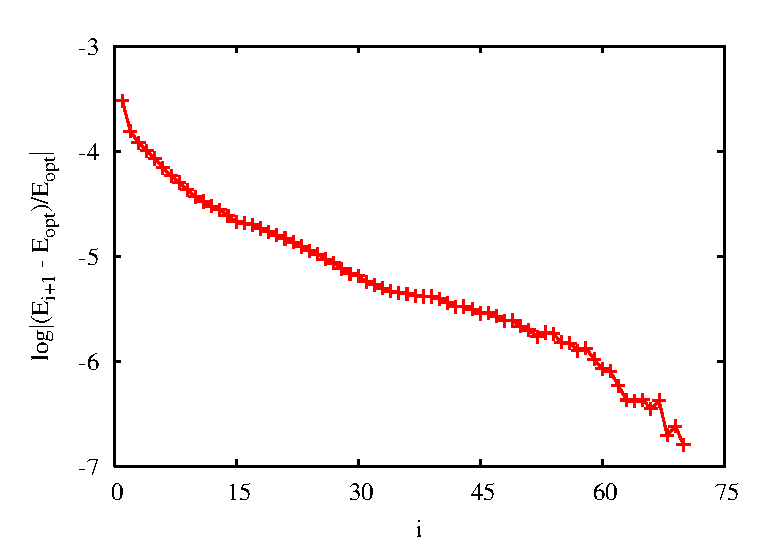
\includegraphics{curve3.eps}}
\resizebox*{3.5in}{!}{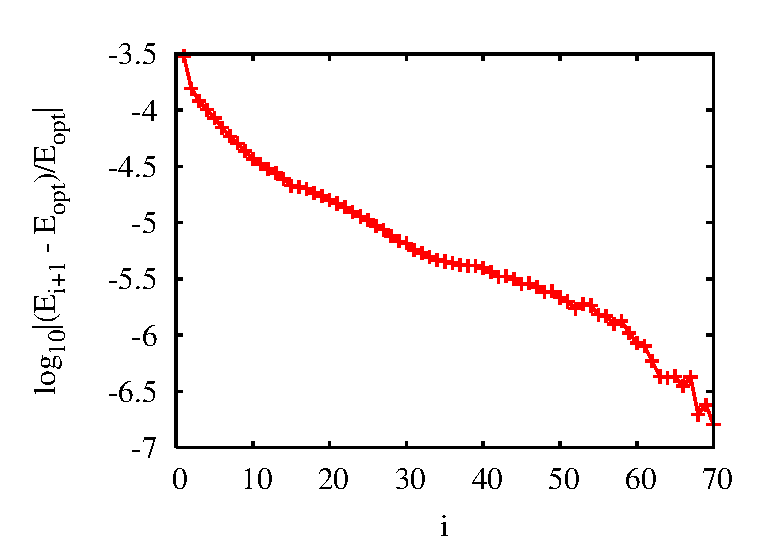
\includegraphics{curve2_1.eps}}
\caption{
\small  
The error of the energy has an exponential decline during
the optimization of a 257 atom protein kinase A fragment. 
$i$ denotes the serial number of steps,
$E_{opt}$ is the optimum energy.
\label{logn-logde}
}
\end{figure}
%
%
%
%
\begin{figure}[h]
%\resizebox*{3.5in}{!}{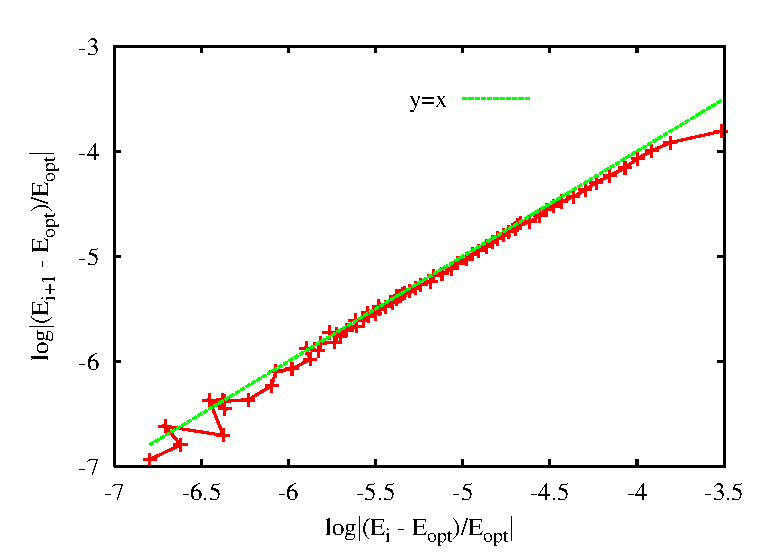
\includegraphics{curve2.eps}}
\resizebox*{3.5in}{!}{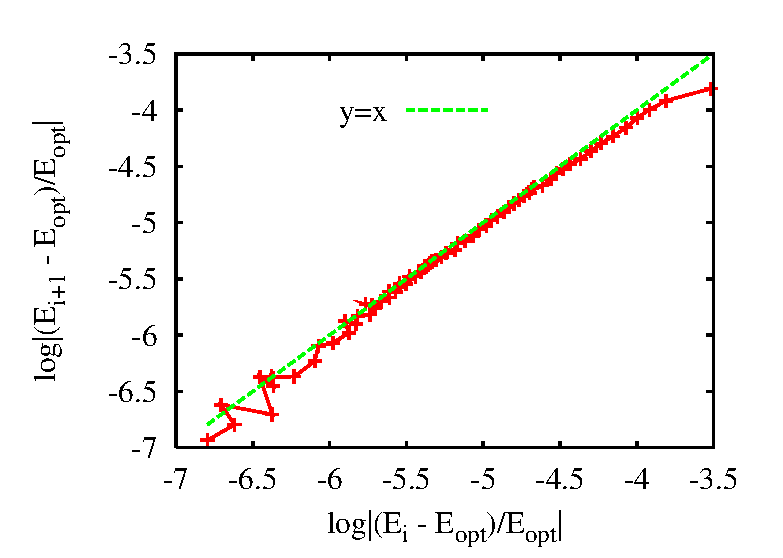
\includegraphics{curve3_1.eps}}
\caption{
\small  
Relative errors of the energy show linear improvement.
Thus, the convergence is of first order. Better, superlinear
convergence can be expected only beyond the $1\times10^{-4}$ Hartree
energy resolution for this molecular size.
\label{order-of-conv}
}
\end{figure}

\section{Summary}
In this article we have presented a new concept
for the optimization of molecular structures.
We have shown, that internal coordinates representing chemical 
entities can efficiently be optimized, without
ever accounting for explicite vibrational couplings, as traditional
optimization techniques do. This allowes an efficient
extension of quantum-level modeling to geometrical processes
of biomolecules, such as enzymatic reactions, macroscopic quantum 
effects in ion-channels or solvent effects on biomolecules.
Our technique can also be used
to provide simple and accurate updates of force-fields
for molecular dynamics simulations, based on the availability of
quantum-mechanical forces.

\begin{acknowledgments}
K. N{\'e}meth gratefully acknowledges to 
{\"{O}}. Farkas (Budapest) for 
providing the Cartesian coordinates of the Baker's test set and to
B.P. Uberuaga (Los Alamos) for calling our attention to Ref. 
\cite{force-matching}.
\end{acknowledgments}

\bibliography{mondo_new}
\end{document}
